%!TEX encoding = UTF-8 Unicode

\documentclass[a4]{article}

\usepackage{pgfplots}

\begin{document}

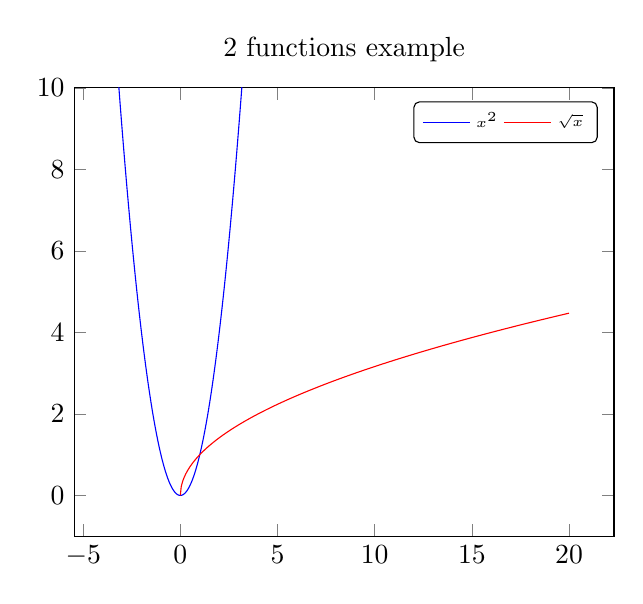
\begin{tikzpicture}
\begin{axis}[
	ymax=10, 
	legend cell align = center,
	legend style={legend pos=north east,
		font=\tiny,
		legend columns=2,
       rounded corners=2pt},
	title=2 functions example]
	\legend{$x^2$,$\sqrt{x}$};
	\addplot[blue,samples=200]{x^2};
	\addplot[red,domain=0:20,samples=500]{sqrt(x)};
\end{axis}
\end{tikzpicture}


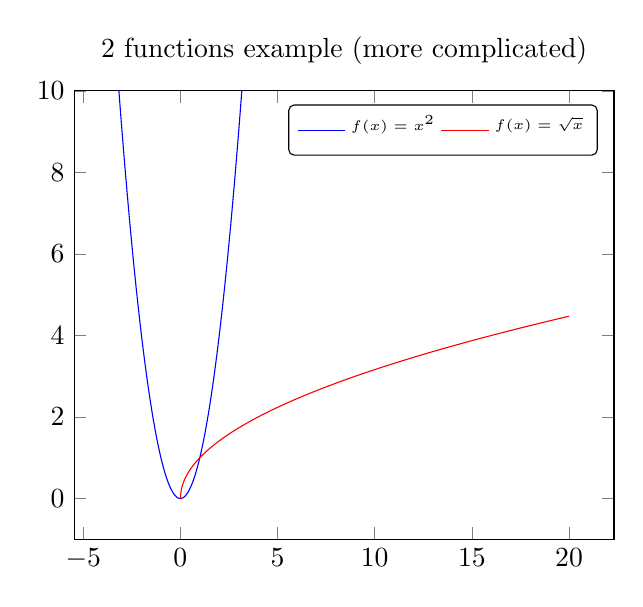
\begin{tikzpicture}
\begin{axis}[
	ymax=10, 
	legend cell align = center,
	legend style={legend pos=north east,
		font=\tiny,
		legend columns=2,
       rounded corners=2pt},
	title=2 functions example (more complicated)]
	\addlegendentry{\raisebox{0.5em}{$f(x)=x^2$}};
	\addlegendentry{\raisebox{0.5em}{$f(x)=\sqrt{x}$}};
	\addplot[blue,samples=200]{x^2};
	\addplot[red,domain=0:20,samples=500]{sqrt(x)};
\end{axis}
\end{tikzpicture}

\end{document}